\subsection{External Interface Requirements}
\begin{itemize}
	\item The user module interface will provide the user with a clean and smart design, which will make it easy for the user to access the system and logon or register with no unwanted constraints.
	\item The user will only be allowed to access his/her application via a smartphone or tablet. The software will work on any operating system. 
        \item The application will be able to fit all screen resolutions with screen rotation capabilities.
	\item When the user logs in or register, his/her information will be sent to a server which will then connect to a database that will either validate the user’s credentials or add the credentials to the system.
	\item To meet disability requirements, users can use the accessibility function that is built into almost all smartphones and tablets.
\end{itemize}
\subsection{Performance Requirements}
\begin{itemize}
	\item The user system will get from 20 000 to 40 000 login requests a day. This branches of into registered students logging into the system more than once a day and guests registering and logging into the system
	\item The user system will have at most 1000 guests using the application on the campus but this value varies in the beginning of the year because most first year have not registered within the first few weeks of the academic year. 
        \item The user system might slow down depending on how the database is implemented and how big it will be but the design patterns used help improve database efficiency and improves server response time.
\end{itemize}
\subsection{Design Constraints}
\begin{enumerate}
	\item Query caching
	\newline
	In order to avoid traffic requests to the database and to speed up database , query caching is crucial. AdoDB provides powerful caching system which can implemented in the navUP system and help improve speed regarding interaction between front end and database.
\end{enumerate}
\subsection{Software System Attributes}

	\subsubsection{Security}
	The navUP system will need to adhere to the highest security standards because of the personal information of users that will be stored. In order to achieve security , The navUP system needs to store users’ information and the passwords should be stored in the database as encrypted to remain hidden from the unauthorised users  .
	\subsubsection{Performance}
	The system should ensure that basic operations like user registration , user login should be of maximum speed. 
	\subsubsection{Availability}
	The navUP system will need to be connected to the internet to ensure that the system can communicate with  the database.
	\subsubsection{Reliability}
	The navUP system will need to work roburstly without any failures including failure to retrieve information from the database.

\subsection{UML diagrams}
\subsubsection{Class diagram}
\begin{figure}[H]
	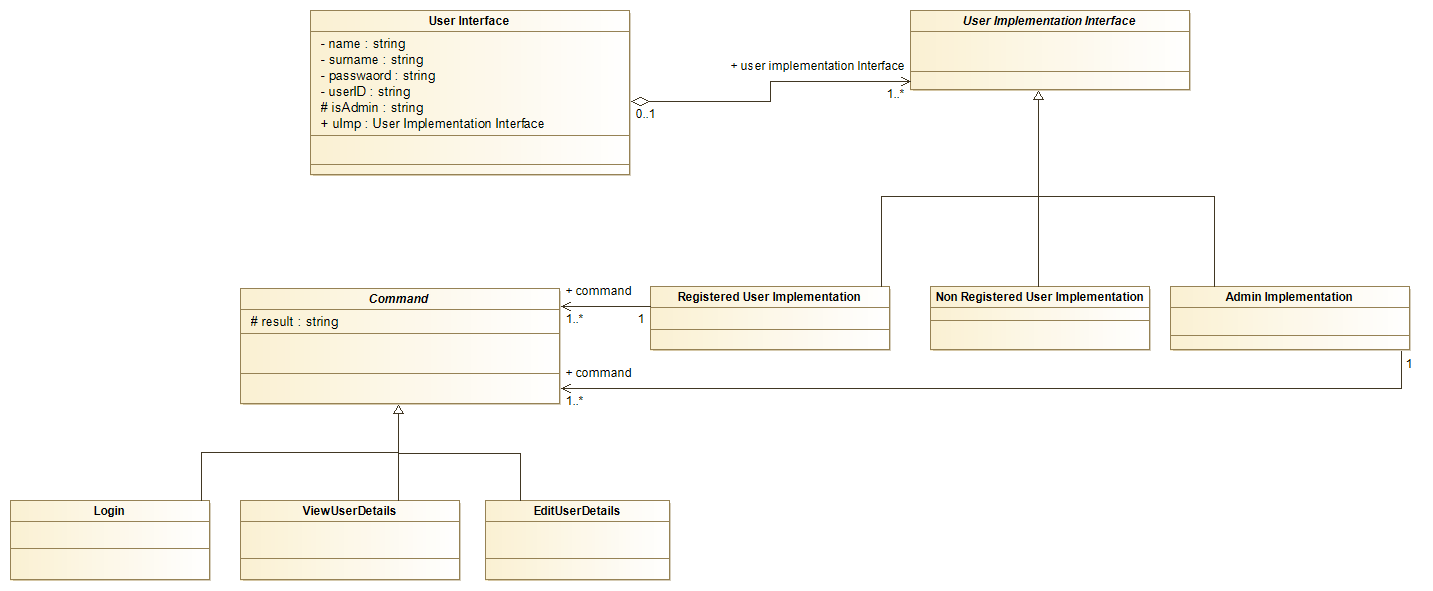
\includegraphics[width=12cm,height=26cm,keepaspectratio]{Users/Pictures/User_Class_Diagram.png}
	\caption{Class diagram for user management module}\label{visina8}
\end{figure}
\paragraph{Discussion of design patterns implemented in UML diagrams:}
		In the user class diagram, I used the bridge design pattern combined with the command pattern. I used the bridge pattern because it maintains a stable client interface while allowing the implementations change. Thus, when a Non-Registered user registers then the implementation can change to registered user implementation and the client will not be affected by the changes in implementation. The client does not know which concrete implementation is being used which is good in terms of security so the client cannot damage the system. The command pattern is used to allow the for requests to be encapsulated which reduces the code size and it allows the operations to be executed in different ways. The requests can be queued and executed later which is useful in increasing the performance of operations. By decoupling the operations is reduces the amount of request that it will have with the database thus, making it more efficient and making the other database operations run faster.
		
\subsubsection{Sequence diagram}
\begin{figure}[H]
	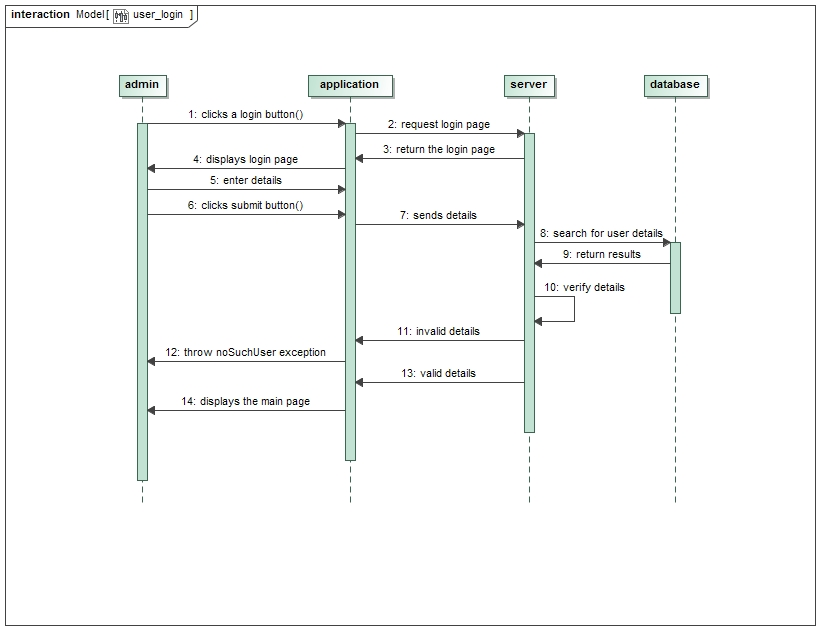
\includegraphics[width=12cm,height=26cm,keepaspectratio]{Users/Pictures/user_sequence_diagram.png}
	\caption{Sequence diagram for user management module}\label{visina8}
\end{figure}

\subsubsection{Activity diagram}
\begin{figure}[H]
	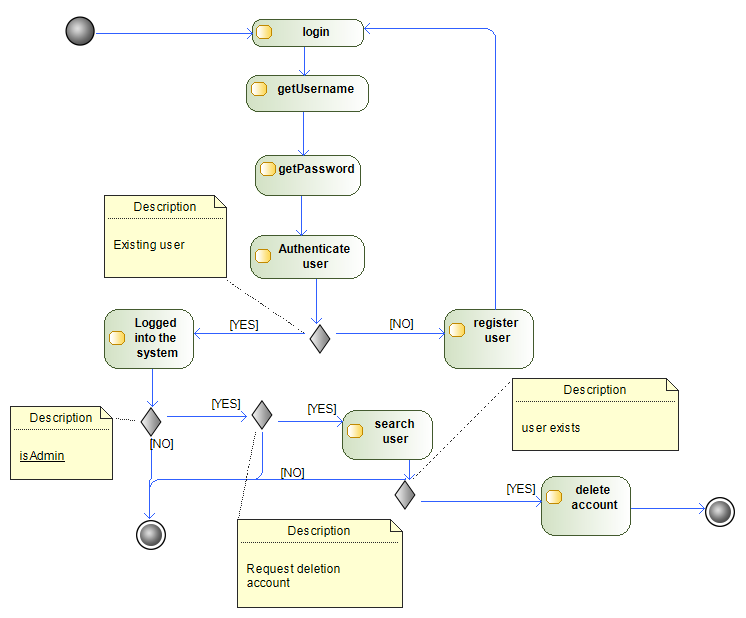
\includegraphics[width=12cm,height=26cm,keepaspectratio]{Users/Pictures/user_Activity_diagram.png}
	\caption{Activity diagram for user management module}\label{visina8}
\end{figure}
\subsubsection{State diagram}
\begin{figure}[H]
	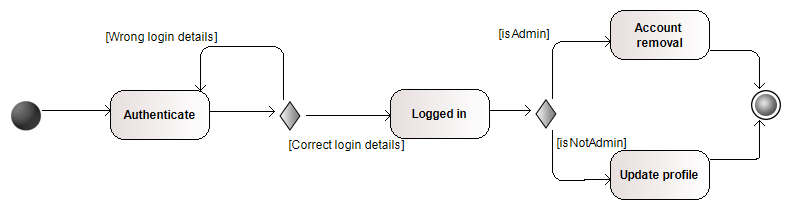
\includegraphics[width=12cm,height=26cm,keepaspectratio]{Users/Pictures/User_State_Diagram.png}
	\caption{State diagram for user management module}\label{visina8}
\end{figure}
\subsubsection{Use Case diagram}
\begin{figure}[H]
	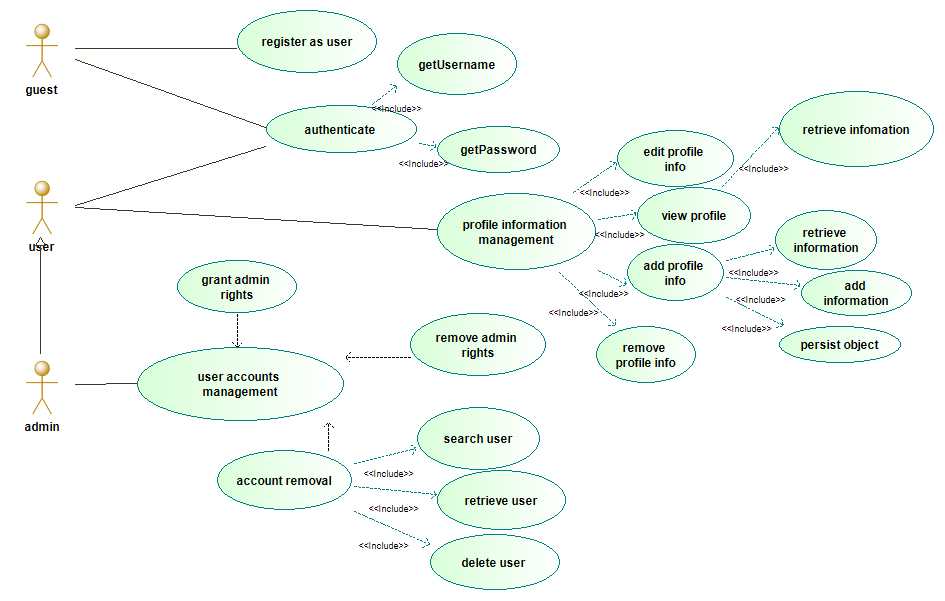
\includegraphics[width=12cm,height=26cm,keepaspectratio]{Users/Pictures/user_use_case_diagram.png}
	\caption{Use case diagram for user management module}\label{visina8}
\end{figure}
